%% Template article for Elsevier's document class `elsarticle'
%% with numbered style bibliographic references
\documentclass[preprint,12pt]{elsarticle}

% remove preprint footnote
\makeatletter
\def\ps@pprintTitle{%
 \let\@oddhead\@empty
 \let\@evenhead\@empty
 \def\@oddfoot{\centerline{\thepage}}%
 \let\@evenfoot\@oddfoot}
\makeatother


\usepackage{setspace}
\doublespacing

\usepackage{hyperref} % auto detect ref type
\usepackage{natbib}
\setcitestyle{authoryear}

%% Use the option review to obtain double line spacing
%% \documentclass[preprint,review,12pt]{elsarticle}

%% Use the options 1p,twocolumn; 3p; 3p,twocolumn; 5p; or 5p,twocolumn
%% for a journal layout:
%% \documentclass[final,1p,times]{elsarticle}
%% \documentclass[final,1p,times,twocolumn]{elsarticle}
%% \documentclass[final,3p,times]{elsarticle}
%% \documentclass[final,3p,times,twocolumn]{elsarticle}
%% \documentclass[final,5p,times]{elsarticle}
%% \documentclass[final,5p,times,twocolumn]{elsarticle}

\usepackage{graphicx}
\usepackage{amssymb}
\usepackage{amsmath}
\usepackage{enumerate}
\usepackage{caption}
\usepackage{textcomp}    % for Hawaii characters
%\usepackage{listings}
%\lstset{language=R}
\usepackage[T1]{fontenc}  % tilde in middle in lstlisting
\usepackage[formats]{listings}
\lstset{language=R,
		basicstyle=\ttfamily,
		columns=fixed,
		basewidth=0.5em,
		literate={~}{{$\sim$}}1
		}

\biboptions{comma,round}

% shortcuts
\newcommand{\bbeta}{\boldsymbol{\beta}}
\newcommand{\blambda}{\boldsymbol{\lambda}}
\newcommand{\T}{\intercal}
\newcommand{\bS}{\mathbf{S}}
\newcommand{\bQ}{\mathbf{Q}}
\newcommand{\bSigma}{\boldsymbol{\Sigma}}
\newcommand{\bm}{\boldsymbol}  % bold maths symbols
\newcommand{\tl}{\tilde{\lambda}}   % thinned little lambda
\newcommand{\tL}{\tilde{\Lambda}}  % thinned big lambda

% RJC 09/08/2019 Added shortcuts for Hawaiian words
\newcommand{\akepa}{\textquotesingle\={a}kepa}  % adds Hawaiian diacritical marks
\newcommand{\Akepa}{\textquotesingle\={A}kepa}  % adds Hawaiian diacritical marks
\newcommand{\hawaii}{Hawai\textquotesingle i}   % adds Hawaiian diacritical marks
\DeclareMathOperator*{\argmax}{arg\,max}  % * means _ puts thing beneath operator

\begin{document}
\begin{frontmatter}
\title{One-stage point transect distance sampling using iterated integrated nested Laplace approximations}

%% use the tnoteref command within \title for footnotes;
%% use the tnotetext command for the associated footnote;
%% use the fnref command within \author or \address for footnotes;
%% use the fntext command for the associated footnote;
%% use the corref command within \author for corresponding author footnotes;
%% use the cortext command for the associated footnote;
%% use the ead command for the email address,
%% and the form \ead[url] for the home page:
%%
%% \title{Title\tnoteref{label1}}
%% \tnotetext[label1]{}
%% \author{Name\corref{cor1}\fnref{label2}}
%% \ead{email address}
%% \ead[url]{home page}
%% \fntext[label2]{}
%% \cortext[cor1]{}
%% \address{Address\fnref{label3}}
%% \fntext[label3]{}


%% use optional labels to link authors explicitly to addresses:
%% \author[label1,label2]{<author name>}
%% \address[label1]{<address>}
%% \address[label,2]{<address>}

% RJC 09/08/2019 Added co-authors and affiliations. Note that I used \affil[]{} instead of \address[]{}
\author[1,*]{Andrew E Seaton}
\author[1,2]{Richard J Camp}
\author[3]{Finn Lindgren}
\author[1]{Janine B Illian}
\author[1]{David L Borchers}
\author[1]{David L Miller}      % Ask about co-authoring the manuscript
\author[1]{Len Thomas}          % Ask about co-authoring the manuscript
\author[1]{Stephen T Buckland}  % Ask about co-authoring the manuscript
\author[4]{Steve J Kendall}     % It is Steve's data we are using and I have already mentioned this manuscript to him.

%\address{Centre for Research into Ecological \& Environmental Modelling and School of Mathematics \& Statistics, University of St Andrews, St Andrews, Fife, Scotland}
\address[1]{Centre for Research into Ecological \& Environmental Modelling and School of Mathematics \& Statistics, University of St Andrews, St Andrews, Fife, Scotland}
\address[2]{U. S. Geological Survey, Pacific Island Ecosystems Research Center, P.O. Box 44, \hawaii{} National Park, HI 96718, U.S.A.}
\address[3]{School of Mathematics, University of Edinburgh, Edinburgh, Scotland}
\address[4]{U. S. Fish and Wildlife, Big Island National Wildlife Refuge Complex, 60 Nowelo St., Suite 100, Hilo, HI  96720, U.S.A.}
\address[*]{Correspondence: Andrew E Seaton, Email: aes22@st-andrews.ac.uk}

\begin{abstract}
A New Abstract Goes Here   
\end{abstract}

%\begin{keyword}
%Distance sampling \sep Stochastic partial differential equations \sep Integrated nested Laplace approximation \sep Generalized additive model
%\end{keyword}
\end{frontmatter}

\section{Introduction}

The estimation of the size and spatial distribution of wild populations of animals is a critical objective within ecology and conservation \citep{schwarz_estimating_1999}. Here we present an analysis of wildlife survey data collected on a critically endangered Hawaiian forest bird that aims to meet this objective.  The Hawaiian \akepa{} is an endemic species whose population declined dramatically during the 20th century [[cite??]].  The remaining population is the focus of sustained conservation efforts and monitoring is required to inform decision-makers about changes in the overall abundance and spatial distribution.  This information is critical when making decisions about conservation strategies.  However, answering these questions presents many statistical challenges.  

Firstly, as in many ecological surveys, it is impossible to undertake a census.  The existing population numbers in the thousands and lives in dense forest where logistical and ecological challenges mean a census is not feasible.  For this reason, a monitoring survey must sub-sample in space and time in some way.  For the \akepa{} this takes the form of the Hawaii Forest Bird Survey (HFBS) \citep{scott_HFBS_1986} which is a large-scale, quantitative survey of Hawaiian forest birds.  Annual surveys of the \akepa{} study-region consist of survey points located along randomly located transects.    

Secondly, even at sampled locations, detectability of animals is uncertain.  The \akepa{} survey attempts to estimate detectability using a distance sampling approach \citep{buckland_distance_2015} where for each observation the distance to the observer is recorded.  A parametric form of detection function is assumed to decay with increasing distance and is estimated from the observed distances.  Because of this, answering questions related to the abundance and spatial distribution must involve the estimation of a complex observation process.  

Thirdly, due to the spatial sub-sampling, a key aim of the analysis is the generation of spatial predictions.  However, as is the case in many species distribution models, we usually have reason to believe there are drivers of the spatial distribution for which we have no explanatory covariates.  For the \akepa{} this takes the form of a north-south gradient that has been investigated but for which no clear-cut explanatory cause has been found [[cite here?]].  From a statistical perspective this suggests the use of spatially-structured random effects to account for the missing covariates.

Fourthly, the resulting statistical model is complex and therefore challenging to effectively communicate the results of the analysis to non-statistically trained stakeholders such as conservation managers and policy officers.  In particular we note the challenge of communicating uncertainty in maps of predicted animal density.

In this paper we present an analysis that seeks to address each of these issues by presenting

\begin{enumerate}[(i)]
	\item A model-based spatial point process perspective on point transect distance sampling, representing the observation model as a thinning probability function.
	\item A one-stage approximate Bayesian approach to inference to simultaneously estimate the observation model and spatial distribution.  This is based on iterated model fits using integrated nested Laplace approximations (INLA) \citep{rue_approximate_2009}.
	\item A computationally efficient Gaussian Markov random field (GMRF) spatial effect based on a stochastic partial differential equation approach \citep{lindgren_explicit_2011} to account for missing covariates.
	\item An approach to model evaluation and communication based on sampling from the joint posterior of all model parameters and excursions methods \citep{bolin_excursion_2015} for investigating uncertainty in spatial predictions.
\end{enumerate}

We note that these challenges are generic to many types of wildlife survey data, not only the \akepa{} survey, and can be addressed by a range of possible statistical approaches.  Our analysis here is one possible choice of approach and throughout the remainder of the paper we will highlight differences with existing approaches.  We demonstrate several novel contributions to the problem of species distribution modelling under imperfect detection.  In particular, the point process perspective with incomplete location information, the one-stage approximate Bayesian inference strategy and focus on communicating uncerainty in spatial predictions using excursions are innovations in this area.  We also note that although we use a Bayesian approach, maximum-likelihood frameworks could also have been used.  Finally, we note that many of the themes addressed in this paper apply beyond the field of spatial ecology and will be of interest to the spatial statistics community in general, particularly for applications with complex observation models of latent processes and where spatial predictions are a key output of the analsyis.  

Our aim is to present a full analysis of the data along with discussion on model specification, inference and model evaluation that reveals key issues in the analysis and our strategies to address them.  Our end hope is that the analysis we present here may provide other researchers with similar data structures an awareness of the issues involved and some options for strategies to use in their own analysis.

The rest of the paper proceeds as follows:  (i) we describe in detail the \akepa{} study-region and survey design; (ii) we present the perspective of distance sampling as a thinned point process; (iii) we describe the GMRF random effect and iterated INLA fitting procedure; (iv) we present the results of the analysis and discuss model evaluation and communication.

\section{Study design}

The \hawaii{} \akepa{} (hereafter \akepa{}; \textit{Loxops coccineus}; nomenclature according to \citealp{usfws_akepa_1970}) is an internationally and federally endangered Hawaiian honeycreeper (\citealp{usfws_akepa_1970, birdlife_akepa_2016}) that is endemic to \hawaii{} Island, USA.  Large-scale, quantitative surveys of Hawaiian forest birds and their habitat commenced in the mid-1970s through the Hawaii Forest Bird Survey (HFBS) \citep{scott_HFBS_1986}. Information from the HFBS was used to update the listing and delisting of endangered species, and establish preserves that coincided with native bird hotspots, including Hakalau Forest National Wildlife Refuge on \hawaii{} Island (hereafter Hakalau) that was the first wildlife refuge with the primary purpose to protect, conserve and manage native forests for threatened and endangered bird and plant species. Due to the broad-scale coverage and robust design HFBS has become the baseline to determine changes in bird species distributions, population sizes and trends in density patterns over time.

During the 20th century \akepa{} declined dramatically due to habitat modification \citep{scott_HFBS_1986, pratt_avifaunal_1994},  mosquito-transmitted avian diseases \citep{pratt_avifaunal_1994, atkinson_wildlife_1995}, introduced predators \citep{lepson_akepa_1997}, and food resources competitors \citep{lepson_akepa_1997}. \Akepa{} has a global abundance of approximately 16,200 (95\%CI 10,000\textendash25,200) birds that has been restricted to five spatially distinct populations \citep{judge_akepa_2018}. Hakalau supports the largest \akepa{} population that in 2012 was estimated at more than 11,000 birds \citep{camp_statespace_2016}. Maintaining and expanding the \akepa{} population at Hakalau is a primary conservation concern. Moreover, having unbiased and precise abundance estimates are required by land and resource managers for evaluating management actions and establishing management planning, and policy makers for decision-making processes.

\subsection{Study area and sampling method}

[[Need to update this and the figure with the extended data area]]

Hakalau was established in 1985 to conserve 15,390-ha of montane forest habitat for native forest birds and rainforest plants. Annual forest bird surveys were initiated in 1987 to determine population status and track trends in abundance. Survey points were established along 15 transects following a systematic, random design with points approximately 150 m apart on transects located either 500 or 1,000 m apart. Following \cite{camp_population_2010, camp_statespace_2016}, we restrict our study area to the 3,061 ha open-forest stratum of Hakalau.  The open-forest stratum was previously heavily grazed, and since the removal of cattle in 1988 regeneration has proceeded naturally \citep{maxfield_hakalau_1998}. To the north the study area follows the refuge boundary while to the east it is bounded by a fence line (Fig. \ref{fig:2002studyareapointspt}). The southern boundary was modified from \cite{camp_population_2010} to exclude the non-sampled forested portion of their study area. The west side of the study area is bounded by pasture that is dominated by grass and is unsuitable habitat for \akepa.

\begin{figure}
	\centering
	\includegraphics[scale=0.5]{figures/2002studyareapoints_pt}
	\caption{Study area (light blue) showing the 2002 survey points (black dots) in Hakalau Forest National Wildlife Refuge, \hawaii{} Island.}
	\label{fig:2002studyareapointspt}
\end{figure}

Surveys used point-transect methods, recording horizontal distances from survey points to individually detected birds. Surveys commenced at dawn and continued until 11:00 or halted when weather conditions exceeded prescribed conditions that hindered detecting birds (light rain, and wind and gust strength \textgreater Baufort scale 3). During 8-min counts trained observers recorded the species, exact distance to the nearest meter and detection type for each bird detected, along with the sampling conditions cloud cover, rain, wind strength, gust strength, and time of day each point was surveyed.   \cite{camp_population_2010,camp_statespace_2016} provide a detailed description of Hakalau, the open-forest study area and the bird surveys.

\subsection{Data description}
[[ Need to update this with extended data ]]

For the purposes of our analysis we selected a single survey from the \akepa{} time series that contained on broad sampling of the study area with sufficient numbers of detections to estimate detectability. In 2002, 289 points were sampled using point-transect distance sampling methods within the 3,061 ha open-forest study area of Hakalau (Fig. \ref{fig:2002studyareapointspt}). 276 \akepa{} were detected on 121 point transects. The number of detections within each sampling unit ranged from zero to 6. 


\section{Distance sampling as a thinned point process}

\subsection{Overview of distance sampling methods}

Distance sampling methods aim to estimate abundance by using a spatially explicit sampling design and assumed detection model to estimate the detectability of animals as a function of distance from observer \citep{buckland_advanced_2004, buckland_distance_2015}. In this section we present a brief historical survey of distance sampling approaches and the approaches of combining distance sampling methods with spatially explicit statistical models.  We end by introducing a predecessor to our method and note differences with previous approaches. 

Standard distance sampling approaches use a hybrid of design- and model-based inference to estimate population size where the probability of detection is modelled as a function of distance and a randomized sampling design allows the construction of Horvitz-Thompson-like estimators of animal density \citep{horvitz_generalization_1952,  buckland_advanced_2004}.

More recently, interest has focused on fully model-based approaches that include a spatially explicit model for animal density and allow the use of non-randomized survey designs.  These methods also allow density to be associated with spatially-indexed covariates and abundance can, in principle, be estimated for any subregion within the study area \citep{johnson_model-based_2010, miller_spatial_2013, buckland_model-based_2016}.  

Model-based distance sampling has been implemented in a two-stage modelling framework.  In the first stage, detectability is estimated within each sampling unit.  In the second stage, detections within sampling units are binned into counts and used as the response variable in a generalized additive model framework where the detectability estimates from the first stage are used as an offset.  Due to often sparse nature of wildlife survey data this may require consideration of over- or under-dispersion and zero-inflated distributions.  Negative-binomial and Tweedie distributions are common choices to model the distribution of counts.  This two-stage approach has come under the name \textit{density surface models} and \cite{miller_spatial_2013} provide a review and software package \texttt{dsm} to fit the models.  

A key concern with the two-stage approach is the propagation of the uncertainty from the detectability estimates to the second-stage spatial model.  Early attempts to address this focused on bootstrapping \citep{lahiri_resampling_2003, hedley_spatial_2004} but more recent work has pointed to potential difficulties of the bootstrapping approach, noting the difficulty of choosing the resampling units as well as the challenge of combining smoothers and spatial bootstraps \citep{bravington_reliable_2018-1}. Instead, \cite{bravington_reliable_2018-1}  proposed avoiding bootstrapping by propagating error based on a second-order Taylor approximation of detectability around the first-stage maximum-likelihood estimate.

Concerns about uncertainty propagation can be avoided by one-stage modelling approaches.  In our experience these tend to be developed within a Bayesian framework.  These approaches use data augmentation and to model unobserved individuals or groups and Markov-chain Monte Carlo (MCMC) methods for inference \citep{royle_hierarchical_2008, schmidt_using_2012}.  More recently  \cite{oedekoven_bayesian_2014} provided a one-stage model that avoids data augmention by specifying a combined likelihood of the detection and spatially-explicit count models and incorporated model uncertainty by applying a reversible jump MCMC algorithm.

The only Bayesian one-stage analysis that does not use MCMC is, to the best of our knowledge, \citet{yuan_point_2017} who use the approximate Bayesian method INLA applied to line transect data.  INLA can be an attractive choice when working with spatially-structured random effects in large or complex spatial domains.  The SPDE approach \citep{lindgren_explicit_2011} allows the construction of a sparse prior precision matrix which INLA can exploit for gains in computational efficiency and the finite element methods based on triangulation have been shown to be more efficient than regular lattice based approaches \citep{simpson_going_2016}, especially in applications with complex boundaries such as coastlines. 

\citet{yuan_point_2017} also take a point process perspective and formulate the detection model as a thinning of the full but imperfectly observed point pattern.  Key to their approach was formulating the detection model using a stochastic partial differential equation.  Similar to spline approaches, choosing a B-spline basis and finite element methods results in a sparse prior precision matrix for the detection model coefficients which can then be incorporated into the latent-Gaussian model framework required by INLA.  Downsides to this approach are that it is challenging to mandate a monotonically decreasing detection function.  The authors suggestion to reject any non-monotonically decreasing functions when sampling from the posterior seems unsatisfactory.    

Here we present a similar approach to \citet{yuan_point_2017} in that our models are fitted using INLA.  However, we avoid the SPDE detection model, instead allowing the user to specify a parametric family of detection functions, such as the half-normal.  This will be more familiar to users of traditional distance samplign approaches.  This results in components of the additive predictor that are non-linear in their parameters.  To deal with this we use a method of iterated model fits based on a Taylor expansion of the non-linear model components.  We name this approach \textit{iterated INLA}.  

We also apply the methods to point transect data which require special treatment to account for the fact that the area surveyed increases with increasing distance from the observer.  Our case study is, to the best of our knowledge, the first analysis of point transect distance sampling data formulated as a thinned point process.  However, the point process viewpoint is not new and has been applied numerous times to line transect data \citep{buckland_model-based_2016, johnson_model-based_2010, hedley_spatial_2004,  hogmander_random_1991, stoyan_remark_1982}.  We also further develop the point process viewpoint to allow point process models to be applied to data with incomplete location information.  It is common for distance sampling surveys to only record the distance to the observer and the observer location.  We show how the point process perspective can still handle this type of data even though the exact location of the point cannot be drawn on a map.


\subsection{Model specification}

In this section we introduce the statistical model for the animal locations and observation process, including a detailed description of how this model can be represented as a modified Poisson likelihood.  We use this formulation to fit the model using the software package \texttt{inlabru} \citep{bachl_inlabru_2019}, an extension to the \texttt{R-INLA} implementation of INLA.

We assume the location of animals are a point pattern that follows a log-Gaussian Cox process with intensity process $\lambda(s)$.  The log-Gaussian Cox process is a flexible approach that can include spatially structured random effects on the intensity process to account for unexplained heterogeneity not captured by fixed-effect covariates.

\sloppy For the case with imperfect detection of points we specify a thinning probability function $g(s) = \mathbb{P}(\text{a point at $s$ is detected})$. A key property of the log-Gaussian Cox process is that a realisation of a point process with intensity process $\lambda(s)$ that is thinned by thinning probability function $g(s)$ also follows a log-Gaussian Cox process with intensity given by $\tl(s) = \lambda(s)g(s)$.

Standard distance sampling approaches specify $g(s)$ as a function that decays with increasing distance.  The distance measured depends on the type of survey.  For line transects the perpendicular distance to the transect line is used.  For point transects the horizontal distance to the observer is the relevant distance.  For the remainder of the paper we assume a point transect survey design.  

The thinning probability function $g(s)$ is specified as a member of a parametric family of functions.  In this paper we demonstrate our approach using the half-normal formulation, although others such as hazard rate, are also common.  If $r(s)$ denotes the distance of a point at $s$ from the observer, the half-normal thinning probability function is $g(s | \sigma) = \exp(-r(s)^2 / 2\sigma^2)$ where $\sigma$ is a variance parameter to be estimated.  The parameter $\sigma$ can only be estimated if an assumption is made about the intensity of the animal locations.  Without such an assumption detectability and intensity are confounded.  The standard assumption in distance sampling is that the intensity is constant with respect to changes in $r(s)$.  Thus any observed differences from uniformity can be attributed to detectability and not variation in the intensity.

A point transect distance sampling survey consists of a set of $K$ sampling units.  The $k$-th sample unit we denote $\Omega_k \subset \mathbb{R}^2$ and the total surveyed region $\Omega = \cup_{k=1}^K \Omega_k$.  For simplicity we assume that all sampling units are discs with radius $W$ and $\Omega_j \cap \Omega_k = \emptyset$ for all $j \neq k$.  The thinning probability function $g(s)$ is defined relative to the positions of the sample units.  The probability of observing a point at location $s$ in the $k$-th sampling unit $\Omega_k$ we denote $g_k(s)$.  The probability of observing a point outside the surveyed region is zero.
Since the surveyed regions are non-overlapping each location $s \in \Omega$ is unambigiously associated with a single thinning probability function $g_k$.  For example, for an observer at location $s_k \in \Omega_k$, the half-normal thinning probability function is $g_k(s) = \exp(-\lVert s - s_k \rVert_2^2 / 2\sigma^2)$. The assumption of non-overlapping survey regions can be relaxed by including extra information such as the time of each observation but, for simplicity, we do not consider this here.  The thinning probability function for any $s \in \Omega$ is then given by $g(s) = g_{k(s)}(s)$ where $k(s) = k$ for $s \in \Omega_k$.

The thinned log-Gaussian Cox process likelihood with observed points at locations $\bm{Y} = (s_1, \ldots, s_n)^\intercal$ is then
\begin{equation}
\label{lgcp-likelihood}
\pi(\bm{Y}) = \exp\left(-\int\displaylimits_{s \in \Omega} \lambda(s) g(s) \mathrm{d}s \right)\prod_{i=1}^n \lambda(s_i)g(s_i)
\end{equation}
where we have suppressed parameter vector notation.  The integral component of the likelihood does not usually have analytical solutions.  Replacing the integral with a weighted sum allows the log-likelihood to be rewritten as a weighted Poisson log-likelihood, which we describe below, adapting the approach of \cite{simpson_going_2016} for a fully observed point pattern.

To evaluate the integral we introduce polar coordinates notation $s_k(r, \theta) = s_k + r\left[\cos\theta, \sin\theta \right]^T$ to represent locations in each sampling unit $\Omega_k$.   In general the thinning function depends only on $r$ and not on $\theta$.  We assume this is the case in the following and use the shorthand $g_k(r) = g(s_k(r, \theta))$. It follows that the integral can be rewritten as a sum of weighted one-dimensional integrals $\sum_{k=1}^K 2\pi \lambda(s_k) \int_0^W r g_k(r)\mathrm{d}r$ using the assumption that $\lambda(s)$ is constant within each sampling unit.  For each sampling unit we approximate the one-dimensional integral using a midpoint integration method with $M$ integration locations $r_{k1}, \ldots, r_{kM}$ and associated weights $\alpha_{k1}, \ldots, \alpha_{kM}$.  This gives
\begin{equation*}
	\int\displaylimits_{s \in \Omega} \lambda(s)g(s)\mathrm{d}s \approx \sum_{k=1}^K \sum_{j=1}^M \tilde{\alpha}_{kj} \tl(s_{kj})
\end{equation*}
where $\tilde{\alpha}_{kj} = 2\pi \alpha_{kj}r_{kj}$ and $\tl(s_{kj}) = \lambda(s_k) g_k(r_{kj})$.

To simplify notation below we let $\tilde{\alpha}_{k} = (\alpha_{k1}, \ldots, \alpha_{kM})^\intercal$ and $\tilde{\alpha} = (\alpha_1^\intercal, \ldots, \alpha_K^\intercal)^\intercal$.  Similarly let $\tl_k = (\tl(s_{k1}), \ldots, \tl(s_{kM}))^\intercal$, $\tl_{int} = (\tl_1^\intercal, \ldots, \tl_K^\intercal)^\intercal$ and denote the intensity evaluated at the observed locations as $\tl_{obs} = (\tl(s_1), \ldots, \tl(s_n))^\intercal$.  Then the approximate log-likelihood is
\begin{equation}
\label{approx-log-likelihood}
	\log \pi(\bm{Y}) \approx - \tilde{\alpha}^\intercal \tl_{int} + 1^\intercal\log\tl_{obs}
\end{equation}
This approximation can be written as a modified Poisson likelihood.  To see this let $\exp \eta = (\tl_{int}^\intercal, \tl_{obs}^\intercal)^\intercal$,
$\alpha = (\tilde{\alpha}^\intercal, 0_{n \times 1}^\intercal)^\intercal$ and construct a vector of pseudo-observations $y = (0_{KM\times 1}^\intercal, 1_{n \times 1}^\intercal)^\intercal$.  Then the approximate likelihood becomes
\begin{equation}
\pi(\bm{Y}) \approx \prod_{i=1}^{KM + n} \eta_i^{y_i}\exp(-\alpha_i\eta_i)
\end{equation}
This is similar to a Poisson likelihood with a $\log\alpha$ offset and can be specified using the Poisson likelihood implementation available in \texttt{R-INLA}.


\subsection{Intensities for incomplete data}

In the above we assume the data are complete records of animal location.  However, in many distance sampling surveys only the location of the observer and the distance to the observer are recorded.  Data of this type can be analysed within a point process framework by deriving the appropriate intensity function for the incomplete data.

Using the polar coordinates notation given above, for a detected point at location $s_k(r, \theta) \in \Omega_k$ we consider the case where we observe $r$ but not $\theta$.  It follows that the intensity for points at a distance $r$ observed within sampling unit $\Omega_k$ is
\begin{align}
\label{intensity-incomplete}
\tl_k(r) &= \oint\displaylimits_{c_k(r)} \lambda(s)g_k(s)\mathrm{d}s \nonumber \\
&= 2\pi\lambda(s_k)rg_k(r)
\end{align}
 where $c_k(r)$ is a circle of radius $r$ centred at $s_k$ and the second line follows from changing to polar coordinates and the assumption of constant intensity within $\Omega_k$.  This intensity differs from the full data case by including the $2\pi$  term to account for the fact that we do not observe $\theta$ and the additional $r$ term to account for the increasing area surveyed at larger distances.

\section{Iterated INLA}

The log-intensity for observed points (the thinned intensity) is $\log\tl(s) = \log\lambda(s) + \log g(s)$.  This presents a problem since $\log g(s)$ is not typically linear in its parameters. However, for any single set of parameter values $g(s)$ can be viewed as an offset term. If we could specify $g(s)$ as known then we could proceed with an inference approach suitable for additive linear predictors.

\begin{itemize}
 \item Description of iterated INLA here
\end{itemize}

\section{Gaussian Markov random field spatial effect}

Using spatially-structured random effects can be computationally expensive, resulting in dense prior precision matrices.  A key development in this area is the use of Gaussian Markov random field (GMRF) approximations to Gaussian random fields (GRFs).  The link between them is via a stochastic partial differential equation solved using finite element methods \citep{lindgren_explicit_2011}.

To model the intensity of animal locations we use a combination of fixed effects of spatial covariates and a spatially structured random effect.  This allows us to associate our survey data with environmental and ecological conditions that may be relevant to understanding the sdistribution of the species of interest.  For cases where we have insufficient covariates to fully explain the location of animals the spatially structured random effect accounts for additional heterogeneity in the intensity and is required to assume conditional independence between points, given the intensity.

The log-intensity of animal locations is given by
\begin{equation*}
\log \lambda(s) = \beta_0 + \sum_v \beta_v z_v(s) + \xi(s)
\end{equation*}
where $\beta_0$ is an intercept parameter, the $z_v(s)$ are spatially indexed covariates with effect parameters $\beta_v$ and $\xi(s)$ is a zero-mean GRF with Mat\'ern covariance
\begin{equation}
C(s_1,s_2) = \frac{2^{1-\nu}}{4\pi\kappa^2\tau^2\Gamma(\nu)}(\kappa \|s_1-s_2\|)^{\nu}K_\nu(\kappa \|s_1-s_2\|)
\end{equation}
where \(\nu, \kappa, \tau\) are parameters and \(K_{\nu}\) is the modified Bessel function of the second kind.  All three parameters are not simultaneously identifiable \citep{zhang_inconsistent_2004} and it is conventional to assume a value for $\nu$ which controls the mean-square differentiability of the process.  We set $\nu = 1$ which is the default value in \texttt{R-INLA}. [[Would like to justify $\nu = 1$ somehow?]]

We use a GMRF approximation of $\xi(s)$ following the approach of \cite{lindgren_explicit_2011} based on specifying $\xi(s)$ via a SPDE.  Given a finite element mesh on the spatial domain with $L$ nodes and associated piece-wise linear basis functions $\phi_1, \ldots, \phi_L$ we represent the GRF as $\xi(s) = \sum_l \xi_l \phi_l(s)$.  The parameters $\xi_1, \ldots, \xi_L$ form a GMRF with sparse prior precision matrix $\bm{Q}_{\xi} = \frac{1}{\tau^2}\left(\kappa^4\bm{C} + 2\kappa^2\bm{G_1} + \bm{G_2}\right)$ where $\bm{C}$, $\bm{G_1}$, $\bm{G_2}$ are all sparse matrices the elements of which are defined via an approximate solution to a SPDE (see Supplementary material). The parameters $\tau$ and $\kappa$ control the shape and rate of decay of the Mat\'ern covariance function.

\section{Results}

We fitted the models using penalised complexity priors for the hyperparameters of the GMRF \citep{simpson_penalising_2017}, setting $\mathbb{P}(\sigma > 2) = 0.01$ and $\mathbb{P}(\rho < 130) = 0.01$ where $\rho$ is the range of the Mat\'ern covariance.  The value of 130 was selected based on the minimum distance between sampling locations.  Full code for the analysis can be found in the Supplementary materials.  Since only distance to observer was recorded we used the adjusted intensity given in \eqref{intensity-incomplete}.   

The predicted mean of the posterior intensity is shown in \autoref{fig:intensity-mean-cv} along with a map of the coefficient of variation (CV) of the posterior intensity field on a regular prediction grid with cell area of approximately 1.7 hectares.  This shows a region of high intensity in the south and much lower intensity in the north, agreeing with a standard two-stage analysis of the same data (see Supplementary materials).  The CV plot shows that the CV in the posterior intensity field is lower areas with greater sampling effort.  There is clear preferential sampling with more sampling in the south than the north  (see \autoref{fig:2002studyareapointspt}).  In the north estimated intensities are lower which also contributes to larger CV values.
\begin{figure}
	\includegraphics[scale=0.5]{figures/intensity_mean_cv_sd.png}
	\caption{(left) Posterior mean, CV and SD of the intensity}
	\label{fig:intensity-mean-cv}
\end{figure}
The standard deviation maps shows more overall posterior variability in south where intensity is larger.  We also map the lower and upper quantiles corresponding to a 95\% credible interval for each prediction location (\autoref{fig:intensity-quantiles}).
\begin{figure}[h]
	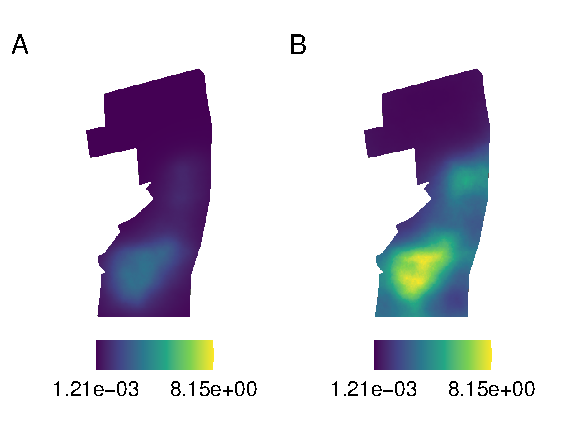
\includegraphics[scale=0.5]{figures/intensity_quantiles.png}
	\caption{The predicted posterior intensity summarised in three plots by the mean (upper),  0.025 quantile (lower left) and 0.975 quantile (lower right) for each prediction grid cell.  All three plots use a common colour scale}
	\label{fig:intensity-quantiles}
\end{figure}

The posterior detection function \autoref{fig:half-normal} shows that detectability drops to just under 0.25 at the maximum observable distance of 60 metres.
\begin{figure}[h]
	\includegraphics[scale=0.5]{figures/halfnormal.png}
	\caption{Posterior detection function.  Black line - mean posterior estimate, grey shaded area - 95\% credible interval}
	\label{fig:half-normal}
\end{figure}

The posterior Mat\'ern correlation function is shown in \autoref{fig:matern-posterior}, the grey regions show the 95\% credible interval. 
\begin{figure}[h]
	\includegraphics[scale=0.5]{figures/matern_posterior.png}
	\caption{Posterior Mat\'ern correlation function}
	\label{fig:matern-posterior}
\end{figure}
Note that this correlation function shows positive correlation even at distances of 10,000 metres, wider than the full length of the study region (approximately 8,000 metres).  This is the correlation on the log-intensity scale.  [[Can I make a better "range of correlation" plot for the posterior intensity process?]]

To further investigate the ability of the GMRF component to capture the heterogeneity we generated 100 thinned point patterns from the fitted model and calculated the pairwise distances between all observations \autoref{fig:post-pp-distances}.  
\begin{figure}[h]
	\includegraphics[scale=0.6]{figures/post_pp_distances.png}
	\caption{Boxplots of frequency of pairwise distances (tick mark values for end of each bin) based on 100 posterior samples.  Red circles: observed frequency of pairwise distances between observations}
	\label{fig:post-pp-distances}
\end{figure}
The plot shows that the GMRF component captures the relevant scale of clustering in the observed data.

We plot the posterior abundance estimate using a monte-carlo method.  Let $n$ denote the abundance of the population within the region of interest and $N = \int_{\Omega}\lambda(s)\mathrm{d}s$ its corresponding random variable within our Bayesian framework.  Integrating the mean of the posterior intensity field provides a point estimate for the abundance - the expected abundance.  We approximate the $\pi(N | \lambda)$ by a monte-carlo method.  Taking $m$ monte-carlo samples  $\lambda_1, \ldots, \lambda_m$ of the posterior intensity field we estimate the posterior for the abundance as $\pi(N | \lambda) \approx 1 / m \sum_{i=1}^m \pi (N | \lambda = \lambda_i)$. Each $\pi(N | \lambda = \lambda_i)$ is a Poisson probability mass function with rate parameter $\int_{\Omega}\lambda_i(s)\mathrm{d}s$. \autoref{fig:realized-abundance-posterior} shows the approximate posterior for $N$ with $m = 20,000$.  This allows us to estimate the probability for any specific value of realised abundance $n$ by calculating $\pi(N = n | \lambda)$.
\begin{figure}
	\includegraphics[scale=0.6]{figures/realized_abundance_posterior.png}
	\caption{Posterior of realized abundance.  The blue line marks the expected abundance}
	\label{fig:realized-abundance-posterior}
\end{figure}

  
% Add table of estimated model parameters
% Add 95% CI figures for N

\clearpage %sort out figure placements later

\section{Communication of Results}

The results presented above are consistent with a more traditional two-stage model on binned count data.  Our presentation of the results is broadly consistent with approaches taken in the species distribution modelling literature, although maps of predictive uncertainty (\autoref{fig:intensity-mean-cv} and \autoref{fig:intensity-quantiles}) are not always provided.  We note a worrying tendency in the species distribution mapping literature to include maps of point estimates without any accompanying communication of uncertainty.  Where uncertainty maps are provided these tend to be maps of predictive uncertainty such as standard deviation or CV (recent examples include \cite{ fuller_novel_2018, vallejo_responses_2017,bradbury_mapping_2014}) based either on a posterior predictive distribution or bootstrapping.  Another approach is to map quantiles or the probability of exceeding certain thresholds (recent examples \cite{russell_avoidance_2016, wilson_hierarchical_2010}).  In the above, we chose to communicate uncertainty through maps of CV, standard deviation, and the 0.025 and 0.975 quantiles.  Whilst all of these maps are informative and useful in their own way, our intention in this section is to highlight limitations with these maps and suggest ways to address these limitations.  

Whilst summary maps of random fields are useful, they all can mask certain properties of the random field. The posterior mean, for example, will be smoother than realisations from the posterior.  \autoref{fig:intensity-realizations} shows three such realisations.  Note that each of them has finer-grained spatial structure than is shown in the posterior mean in \autoref{fig:intensity-mean-cv}.  One interpretation of this is that animals will tend to be more clustered than might be expected if we only looked at the posterior mean.
\begin{figure}
	\includegraphics[scale=0.35]{figures/intensity_realized.png}
	\caption{Three realizations of the posterior intensity field}
	\label{fig:intensity-realizations}
\end{figure}
During model evaluation we recommend producing plots of realisations as these will more closely resemble the spatial structure of the observed data.  

The CV map (\autoref{fig:intensity-mean-cv}) can be hard to interpret in regions of low estimated intensity.  If the posterior standard deviation is relatively consistent across the survey region, CV values will be higher in regions of low predicted intensity.  The observed patterns in such maps will highlight regions of relatively lower intensity, not necessarily higher uncertainty.  This is problem is further confounded in the case with spatially varying posterior standard deviation.

The quantile maps also suffer from a potential difficulty in interpretation. The temptation is to interpet the maps as showing possible intensity surfaces that could have produced the observed data.  Presenting these quantiles side by side in a single map obscures the fact that it is vanishingly unlikely for all prediction values to simultaneously achieve the 0.025 or 0.975 quantile.  A similar problem will occur with mapping the marginal probability of exceeding a threshold at each prediction locations.  We believe most non-statistically trained audiences will struggle with this caveat to interpeting the map.  To demonstrate the possible consequences of this we treated the lower and upper quantile plots as though they were intensities and integrated them to obtain an expected abundance estimate of approximately 3,300 for the 0.025 quantile map and 12,400 for the 0.975 quantile map.  A naive (and tempting) interpretation of these numbers is as lower and upper limits of the 95\% credible interval for abundance. However, these abundance estimates are outside the support of the posterior for abundance (see \autoref{fig:realized-abundance-posterior}).  This demonstrates that the natural tendency to interpet these maps as possible intensities leads to interpretations that are inconsistent with the very model that generated the maps.

For the standard deviation map care should be given to what the mapped values imply in the context of a given analysis.  A default colour scale will more or less always show some spatial variation in uncertainty, with some regions of relatively high or low uncertainty.  What such a map does not show is whether these values actually matter in the context of the analysis.  For example, it could be the case that the standard deviation values are so large as to make the predictions operationally useless everywhere.  Or, on the other end of the scale, perhaps differences between high and low uncertainty regions (`high' and `low' as defined by some default colour scale) are small enough to be negligible when it comes to decision making, in which case such a spatially varying map is not a relevant output of the analysis.  These are two extreme examples, cases in between suffer from the same problem.  

Our solution to the problems in the quantile and standard deviation maps is to suggest that consideration should be given \emph{a priori} to values of the process and levels of uncertainty that are important and suitable given the context of the analysis.  These values can then be used to construct summary maps.  We demonstrate this perspective through the use of excursions sets and functions \citep{bolin_excursion_2015}, although there are many possible approaches.  These techniques require the user to specify thresholds of interest for the process itself and acceptable levels of uncertainty. 

This approach to representing variability in stochastic processes specifically considers the joint probability of events across multiple locations.  The positive excursion set with level $u$ for a function $f(s)$ with domain $\Omega$ is $A_u^{+}(f) = \{ s \in \Omega ; f(s) > u \}$ i.e. the set of all locations in $\Omega$ where $f$ exceeds the a threshold value $u$. For a stochastic process $\lambda(s)$ the positive excursion set with level $u$ and probability $1 - \alpha$ is
\begin{equation*}
E_{u,\alpha}^{+}(\lambda) = \argmax_{D}\{\lvert D \rvert : \mathbb{P}\left[D \subset A_u^{+}(\lambda)\right] \geq 1 - \alpha \}
\end{equation*}
Note that $A_u^{+}(f)$ specifies a set for which a function $f(s)$ exceeds a threshold value $u$ for \textit{every location} in the set.  As such the positive excursion set $E_{u,\alpha}^{+}(\lambda)$ is the largest such set for which a threshold is exceeded simultaneously for all locations in the set.  Negative excursion sets can be similarly defined.  Excursion sets can be estimated by considering candidate sets for $D$ of increasing size and a sequential integration scheme to estimate probabilities.  An implementation is available in the \texttt{excursions} package \citep{bolin_calculating_2018} available through the Comprehensive R Archive Network \citep{r_2017}.

\autoref{fig:excursions} (left panel) shows the positive excursion set with a level corresponding to 1 bird per hectare with probability 0.95.  This figure can be interpreted in a natural way.  It is the largest region for which the intensity is greater than 1 bird per hectare for every location within the region, with probability 0.95.
\begin{figure}
	\includegraphics[scale=0.5]{figures/excursions.png}
	\caption{Left:  The positive excursion set with a level corresponding to 1 bird per hectare and probability 0.95.  Right: The positive excursion function with a level corresponding to 1 bird per hectare}
	\label{fig:excursions}
\end{figure}
To visualise multiple such maps we can use the excursion function $F_u^{+}(s) = \sup \{1 - \alpha ; s \in E_{u,\alpha}^+ \}$, which defines for each location something similar to a p-value.  For each $s$ it is the largest possible probability $1 -\alpha$ for which that location would be in the excursion set defined using probability $1 - \alpha$.  The excursion function with a level corresponding to 1 bird per hectare is shown in \autoref{fig:excursions} (right panel).  This figure can also be interpreted naturally.  It shows the largest possible probability for each location to be a member of a set in which the intensity exceeds a threshold simultaneously across all locations in the set. It is clear from the figure that regions on the edge of the excursion set would be included if the $\alpha$ value were allowed to increase slightly.  However, for regions in the north there is essentially no probability level for which those locations would be included in $A_u^{+}(\lambda)$.  
We chose the threshold of 1 bird per hectare and an error probability of 0.05 to demonstrate the approach.  Multiple values for each of these can be considered as a simple extension.


\section{Discussion}

Our intention in this paper was to present a new approach to analysing point transect distance sampling data that incorporates several innovative new methods and considers the entire workflow of model specification, inference, evaluation and communication of results.  Although each of these areas are substantive enough to be the main focus of a paper, we hope our brief presentation of issues that arise in each area and our chosen solutions will be useful to statisticians who face similar questions and data structures.

There are several natural extensions to the model.  For this analysis we only considered a single survey year.  Spatio-temporal extensions to this are possible, for example by considering a space-time interaction models.  \texttt{R-INLA} has the ability to fit space-time effects that can be represented as a kronecker product of the relevant precision matrices.  An example of this type of space-time interaction effect would be the spatial SPDE above interacting with an AR1 temporal process.  \cite{blangiardo_spatial_2013} show how this can be done with numerous examples and code snippets.    

Another extension is to consider more complicated observation processes.  For example, we did not use any explanatory covariates for the detection function.  This remains to be investigated further.  Any additional parameters to the detection function would result in a higher-dimensional outer optimisation problem for iterated INLA.  This could lead to problem if, for example, identifiability is an issue.  

We note also that our presentation of abundance estimates differs from typical presentations.  It is common to report a point estimate of the expected abundance and uncertainty in this point estimate.  However, uncertainty in a point estimate will tend to have lower variance than variance of the random variable of interest.  We find the distinction between expected and realised abundance to be a useful one. The credible intervals for the posterior expected abundance will be narrower than the credible intervals for the posterior realised abundance.  The Bayesian perspective is useful here as well as for the uncertainty in the detection model estimates.  Since outputs based on sampling from the joint posterior of all model parameters, including the detection model, the Bayesian framework means the resulting model outputs we present here naturally average over the uncertainty in the observation process.  [[Not really sure if this stuff is worth mentioning or if can be said in a better way]]

Our use of \texttt{inlabru} and \texttt{R-INLA} for inference means we can take advantage of the sparsity of the GMRF precision matrix, a key advantage of the SPDE approach.  A dense covariance matrix of dimension $n \times n$ typically has an $\mathcal{O}(n^3)$ cost to invert.  In contrast to this \texttt{R-INLA} makes use of sparse matrix algorithms to invert a sparse 2-dimensional precision matrix at a typical cost of $\mathcal{O}(n^{3/2})$ \citep{lindgren_explicit_2011}.  This computational efficienty, in addition to the flexibility of the mesh triangulation, can make the SPDE an attractive choice for implementing high-resolution spatial effects in complex domains.  An additional benefit, as described in detail in \cite{yuan_point_2017}, is that the SPDE can also be implemented on the sphere, making analysis of global datasets computationally feasible.

In our analysis we only briefly touch upon the problem of communicating uncertainty in maps and highlight the excursions methods as a new and positive addition to this area.  Our example threshold was chosen arbitrarily and it is not obvious to us that there will always be an easy or simple choice of thresholds and levels of uncertainty for a given analysis.  This requires the input of relevant domain expertise and statistical knowledge so stakeholders understand the consequences of the thresholds and uncertainty levels they wish to consider.  The most important consequences of an analysis are the possible conclusions and decisions that will be taken on the basis of the results.  Here we advocate the view that model estimates should be converted into outputs, with associated uncertainty, that are most directly relevant to these conclusions.  In the above we chose to use excursion sets, excursion functions and the posterior of realised abundance as a demonstration of this.  It is not always the case that a map of predicted mean abundance will be the best output for a species distribution model.  

The point process perspective with spatial SPDE effect can seem fundamentally different to a two-stage GAM approach.  However, we think that it can be useful to highlight the similarities in approach.  It can be tempting to think that because with the point process model does not require us to bin the data into counts that we can avoid some loss of information.  However, we also had to make the same assumption of constant intensity within each transect that is common in more traditional distance sampling approaches.  This means the exactly location of the points is not used to inform the posterior intensity.  The assumption of constant intensity within each point transect is essentially the point process version of binning point data into counts.

The SPDE effect can also seem fundamentally different to, say, a spline-based smoother.  However, there is a fundamental connection between SPDEs and optimal smoothing splines.  The optimal smoothing spline is a lminimum variance unbiased linear estimator of the posterior mean of an SPDE \citep{kimeldorf_spline_2002}.  This means a smoothing spline can be interpreted as an SPDE and vice-versa.  Depending on the methods a user is most familiar with this can be a useful perspective.  \cite{yue_bayesian_2014} show how to implement common spline penalties in an SPDE framework and \cite{miller_understanding_2019} offer a complementary explanation to interpret and fit SPDE models within standard penalised regression splines software.

\clearpage
\bibliographystyle{chicago}
\bibliography{paper}

\end{document}